\section{Expression textuelle des exigences}


%\subsection{}
%\paragraph{}

\subsection{Description du système et de son environnement}
\begin{figure}[H]
	\begin{center}	
		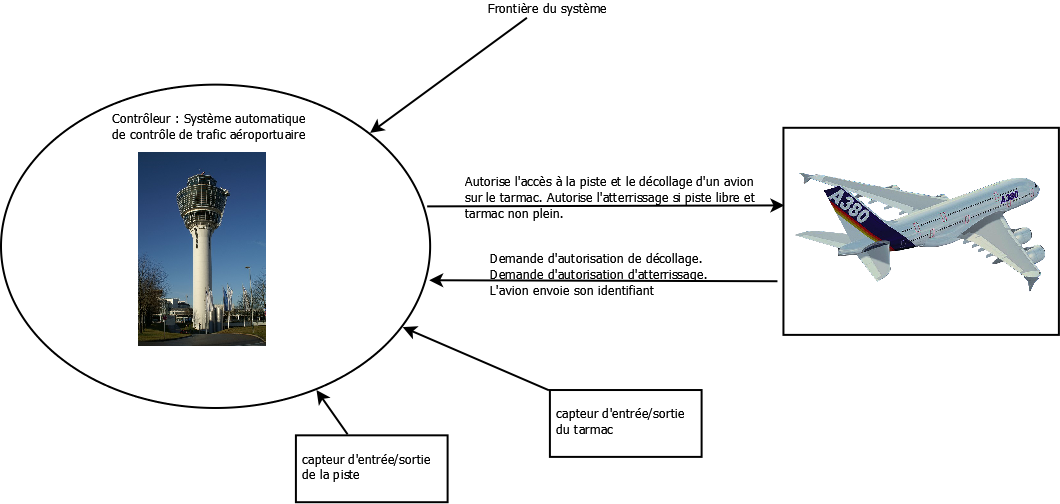
\includegraphics[scale=0.3]{images/ctx}
		\caption{Diagramme hiérarchique des fonctions}
		\label{ctx}
	\end{center}
\end{figure}


\subsection{Analyse des spécifications}

\paragraph{}

Le système à concevoir est un \textbf{contrôleur aérien automatique} chargé de contrôler le trafic sur le tarmac et d'autoriser l'accès à la piste des avions prêts au décollage. 
\paragraph{}
Ce système est un logiciel qu'on appelera le Contrôleur. Ce contrôleur interagit avec son environnement à savoir les pilotes et des capteurs non précisés dans l'énoncé. Les spécifications sont incomplètes car le contrôleur doit forcément autoriser ou refuser les avions à l'atterrissage également. Il est nécessaire d'avoir un capteur qui permet de compter les avions qui entrent et sortent du tarmac et un autre capteur qui assure le comptage des avions sur la piste. Les avions ne peuvent atterrir que si l'aéroport n'est pas plein, 20 places maximum sont disponibles. 
\paragraph{}
On suppose que les clearances sont données aux avions qui se trouvent sur le tarmac. Dès l'autorisation de décoller donnée, l'avion se rend sur la piste et décolle. Il n'y a pas d'étape intermédiaire. Un système de communication sécurisé de type data-link doit exister pour donner les clearances et recevoir les identifiants et les demandes des pilotes.

\paragraph{}
On suppose qu'il ne peut y avoir qu'un seul avion sur la piste ; pas de possibilité
de mettre deux avions au décollage en même temps.


\subsection{Reformulation des exigences}

\begin{table} [H]
	
	\centering
\rowcolors{2}{gray!65}{white}
\begin{tabu}{|[2pt] p{1.7cm} | [2pt]p{15cm}|[2pt]}

	\tabucline[2pt]{-} \rowcolor{yellow}
\Centering	\textbf{Label}& \Centering \textbf{Exigence}  \\ \tabucline[2pt]{-}

	\hline 
	FON-1&Le contrôleur doit autoriser les avions à décoller et atterrir  \\ 
	\hline 
FON-2	& Le nombre d'avions sur le tarmac est limité à 20 y compris ceux en attente  \\ 
	\hline 
	FON-3& Des avions entrent et quittent la piste d'atterrissage décollage  \\ 
	\hline 
	FON-4& Des avions entrent sur le tarmac et le quittent  \\ 
	\hline 
	FON-5& La piste ne peut être occupée par plus de un avion \\ 
	\hline 
	FON-6& Le nombre de décollages ou atterrissages successifs n'est pas limité   \\ 
	\hline 
	FON-7& Le contrôleur doit fixer et délivrer les clearances à l'avance   \\ 
	\hline 
	FON-8& Le contrôleur ne doit autoriser l'avion qu'après l'envoi de son identifiant    \\ 
		\hline
	FON-9& Le contrôleur doit soit refuser, soit accepter, soit mettre en attente l'avion demandeur   \\ 
 	\hline
 FON-10& Le contrôleur doit refuser la clearance après 10 de mise en attente.   \\ 
	\hline 
   ENV-1 &Tout avion se dirigeant vers la piste doit avoir une autorisation de décoller \\ 
   	\hline 
   ENV-2 &Le système est muni d'un capteur qui permet de compter les avions sur la piste \\ 
   \hline 
   ENV-3 &Le système est muni d'un capteur qui permet de compter les avions sur la tarmac \\ 
\tabucline[2pt]{-}
\end{tabu} 
\caption{Tableau des exigences}
\end{table}

